\documentclass[a4paper,12pt, openany]{extbook}
% %%%%%%%%%%%%%%%%%%%%%%%%%%%%%%%%%%%%%%%%%
% % LaTeX Template
% % Version 1.0
% %
% % This template originates from:
% % http://www.LaTeXTemplates.com
% %
% % Authors:
% % Rocco Lo Russo (https://github.com/roccolr)
% %%%%%%%%%%%%%%%%%%%%%%%%%%%%%%%%%%%%%%%%%


%----------------------------------------------------------------------------------------
%	PACKAGES AND OTHER DOCUMENT CONFIGURATIONS
%----------------------------------------------------------------------------------------

\usepackage{amsmath,amsfonts,stmaryrd,amssymb} % Math packages
\usepackage{graphicx}
\usepackage[ddmmyyyy]{datetime}
\usepackage{enumerate} % Custom item numbers for enumerations

\usepackage[ruled]{algorithm2e} % Algorithms

\usepackage[framemethod=tikz]{mdframed} % Allows defining custom boxed/framed environments

\usepackage{listings} % File listings, with syntax highlighting
\usepackage[hidelinks]{hyperref}
\usepackage{wrapfig}

\lstset{
  language=C,
  basicstyle=\ttfamily\small\color{black},
  numbers=left,
  numberstyle=\small\color{gray},
  stepnumber=1,
  numbersep=4pt,
  frame=single,
  rulecolor=\color{black},
  framesep=5pt,
  xleftmargin=20pt,
  framexleftmargin=15pt,
  breaklines=true,
  showstringspaces=false,
  keywordstyle=\color{purple}\bfseries,          % parole chiave (if, else, int, return...)
  commentstyle=\color{teal}\itshape,           % commenti
  stringstyle=\color{orange},                   % stringhe
  identifierstyle=\color{black},                % identificatori normali
  emph={size_t, uint32_t, uint64_t, TAS, RTE},            % tipi aggiuntivi
  emphstyle=\color{blue}\bfseries,            % stile tipi aggiuntivi
  morekeywords={uint8_t, uint16_t, uint32_t, uint64_t, int8_t, int16_t, int32_t, int64_t, bool, true, false}, % tipi e parole chiave extra
  morecomment=[l]{//},                           % commenti con //
  morecomment=[s]{/*}{*/},                       % commenti multilinea
}

\lstdefinelanguage{RISCAsm}{
  morekeywords={
    ADDQ, SUM, ANDI, MOVE,MOVEA, MOVEM, DC, DS, sra, 
    lw, sw, li, la, mv, 
    BEQ, BNE, JMP, CMP, jalr, ret, 
    NOP, lui, RTE, RTS, 
    ecall, ebreak, ORG, EQU, JSR, CLR, TAS 
  },
  sensitive=true,
  morecomment=[l]{\*},
  morestring=[b]",
  basicstyle=\ttfamily\small\color{black},
  keywordstyle=\color{purple}\bfseries,
  commentstyle=\color{teal}\itshape,
  stringstyle=\color{orange},
  numbers=left,
  numberstyle=\small\color{gray},
  stepnumber=1,
  numbersep=4pt,
  frame=single,
  rulecolor=\color{black},
  framesep=5pt,
  xleftmargin=20pt,
  framexleftmargin=15pt,
  showstringspaces=false,
  breaklines=true,
}

%----------------------------------------------------------------------------------------
%	DOCUMENT MARGINS
%----------------------------------------------------------------------------------------

\usepackage{geometry} % Required for adjusting page dimensions and margins

\geometry{
	paper=a4paper, % Paper size, change to letterpaper for US letter size
	top=2.5cm, % Top margin
	bottom=3cm, % Bottom margin
	left=2.5cm, % Left margin
	right=2.5cm, % Right margin
	headheight=14pt, % Header height
	footskip=1.5cm, % Space from the bottom margin to the baseline of the footer
	headsep=1.2cm, % Space from the top margin to the baseline of the header
	%showframe, % Uncomment to show how the type block is set on the page
}

%----------------------------------------------------------------------------------------
%	FONTS
%----------------------------------------------------------------------------------------

\usepackage[utf8]{inputenc} % Required for inputting international characters
\usepackage[T1]{fontenc} % Output font encoding for international characters

\usepackage{XCharter} % Use the XCharter fonts
\usepackage{enumitem}
\usepackage{xcolor}
\usepackage{tikz} 
\usetikzlibrary{positioning}

% pseudocode environment %


%----------------------------------------------------------------------------------------
%	COMMAND LINE ENVIRONMENT
%----------------------------------------------------------------------------------------

% Usage:
% \begin{commandline}
%	\begin{verbatim}
%		$ ls
%		
%		Applications	Desktop	...
%	\end{verbatim}
% \end{commandline}

\mdfdefinestyle{commandline}{
	leftmargin=10pt,
	rightmargin=10pt,
	innerleftmargin=15pt,
	middlelinecolor=black!50!white,
	middlelinewidth=2pt,
	frametitlerule=false,
	backgroundcolor=black!5!white,
	frametitle={Command Line},
	frametitlefont={\normalfont\sffamily\color{white}\hspace{-1em}},
	frametitlebackgroundcolor=black!50!white,
	nobreak,
}

% Define a custom environment for command-line snapshots
\newenvironment{commandline}{
	\medskip
	\begin{mdframed}[style=commandline]
}{
	\end{mdframed}
	\medskip
}

%----------------------------------------------------------------------------------------
%	FILE CONTENTS ENVIRONMENT
%----------------------------------------------------------------------------------------

% Usage:
% \begin{file}[optional filename, defaults to "File"]
%	File contents, for example, with a listings environment
% \end{file}

\mdfdefinestyle{file}{
    innertopmargin=1.6\baselineskip,
    innerbottommargin=0.8\baselineskip,
    topline=false, bottomline=false,
    leftline=false, rightline=false,
    leftmargin=2cm,
    rightmargin=2cm,
    singleextra={
        \draw[fill=black!10!white](P)++(0,-1.2em)rectangle(P-|O);
        \node[anchor=north west] at(P-|O){\ttfamily\mdfilename};
        \def\l{3em}
        \draw(O-|P)++(-\l,0)--++(\l,\l)--(P)--(P-|O)--(O)--cycle;
        \draw(O-|P)++(-\l,0)--++(0,\l)--++(\l,0);
    },
}

% Comando per tab a 4 spazi all’interno dell’ambiente file
\newenvironment{file}[1][File]{%
    \medskip
    \newcommand{\mdfilename}{#1}
    % Rende il carattere tab attivo e lo definisce come 4 spazi
    \catcode`\^^I=\active
    \def^^I{\hspace*{4ex}}%
    \begin{mdframed}[style=file]
}{%
    \end{mdframed}
    \medskip
}

%----------------------------------------------------------------------------------------
%	NUMBERED QUESTIONS ENVIRONMENT
%----------------------------------------------------------------------------------------

% Usage:
% \begin{question}[optional title]
%	Question contents
% \end{question}

\mdfdefinestyle{question}{
	innertopmargin=1.2\baselineskip,
	innerbottommargin=0.8\baselineskip,
	roundcorner=5pt,
	nobreak,
	singleextra={%
		\draw(P-|O)node[xshift=1em,anchor=west,fill=white,draw,rounded corners=5pt]{%
		Question \theQuestion\questionTitle};
	},
}

\newcounter{Question} % Stores the current question number that gets iterated with each new question

% Define a custom environment for numbered questions
\newenvironment{question}[1][\unskip]{
	\bigskip
	\stepcounter{Question}
	\newcommand{\questionTitle}{~#1}
	\begin{mdframed}[style=question]
}{
	\end{mdframed}
	\medskip
}

%----------------------------------------------------------------------------------------
%	WARNING TEXT ENVIRONMENT
%----------------------------------------------------------------------------------------

% Usage:
% \begin{warn}[optional title, defaults to "Warning:"]
%	Contents
% \end{warn}

\mdfdefinestyle{warning}{
	topline=false, bottomline=false,
	leftline=false, rightline=false,
	nobreak,
	singleextra={%
		\draw(P-|O)++(-0.5em,0)node(tmp1){};
		\draw(P-|O)++(0.5em,0)node(tmp2){};
		\fill[black,rotate around={45:(P-|O)}](tmp1)rectangle(tmp2);
		\node at(P-|O){\color{white}\scriptsize\bf !};
		\draw[very thick](P-|O)++(0,-1em)--(O);%--(O-|P);
	}
}

% Define a custom environment for warning text
\newenvironment{warn}[1][Warning:]{ % Set the default warning to "Warning:"
	\medskip
	\begin{mdframed}[style=warning]
		\noindent{\textbf{#1}}
}{
	\end{mdframed}
}

%----------------------------------------------------------------------------------------
%	INFORMATION ENVIRONMENT
%----------------------------------------------------------------------------------------

% Usage:
% \begin{info}[optional title, defaults to "Info:"]
% 	contents
% 	\end{info}

\mdfdefinestyle{info}{%
	topline=false, bottomline=false,
	leftline=false, rightline=false,
	nobreak,
	singleextra={%
		\fill[black](P-|O)circle[radius=0.4em];
		\node at(P-|O){\color{white}\scriptsize\bf i};
		\draw[very thick](P-|O)++(0,-0.8em)--(O);%--(O-|P);
	}
}

% Define a custom environment for information
\newenvironment{info}[1][Info:]{ % Set the default title to "Info:"
	\medskip
	\begin{mdframed}[style=info]
		\noindent{\textbf{#1}}
}{
	\end{mdframed}
}


\hbadness=10000
\hfuzz=50pt % Include the file specifying the document structure and custom commands

% ----------------------------------------------------------------------------------------
% TITOLO
% ----------------------------------------------------------------------------------------
\title{
    
\includegraphics[width=0.4\textwidth]{fig/logo_unina.png} \\ % Modifica 'logo' con il nome del file del tuo logo
    \vspace{1cm}
    \Huge{High Performance and\\Quantum Computing} \\
    \vspace{0.5cm} 
    \Large{Anno Accademico\\2025/26}
}
\author{\textbf{Rocco Lo Russo}\\\textbf{Agostino D'Amora}} % Modifica con il tuo nome
\date{}

% ----------------------------------------------------------------------------------------
\begin{document}


\maketitle

% TAVOLA DEI CONTENUTI
\tableofcontents
\newpage

\chapter*{Introduzione}
In questo documento vengono raccolti appunti del corso \textit{High Performance and Quantum Computing} tenuto nell'anno 2025-26 dal professor Cilardo presso l'università di Napoli Federico II, Dipartimento Ingegneria Elettrica e Tecnologie dell'Informazione.

\noindent \uppercase{è} assolutamente scoraggiata la vendita di questi appunti, che possono in qualsiasi momento essere scaricati gratuitamente da \href{https://github.com/h-tajato/hpqc_notes}{github}. Allo stessa repository è possibile in qualsiasi momento contruibuire seguendo le istruzioni esposte nel README.

\noindent Per la parte iniziale di ricapitolazione, sono stati utilizzati gli appunti raccolti durante il corso di Architettura e Progetto dei Calcolatori tenuto nell'anno 2025-26 dal professor Mazzocca presso l'università Federico II di Napoli (a cui è possibile accedere sia per consultare che per contribuire, nelle stesse modalità, su \href{https://github.com/Agda78/APC-appunti}{github}), i libri \textit{Computer Organization and Desing Patterns} (Hannessy-Patterson) e degli stessi autori \textit{Computer Architecture (a quantitative approach)}.


\chapter{Richiami APC} \label{chap:richiami_apc}
\section{Richiami Pipelining}
Il pipelining è una tecnica di implementazione di processori dove diverse istruzioni si sovrappongono durante l'esecuzione. Questa tecnica, chiave nella progettazione dei moderni processori, trae vantaggio dal parallelismo che esiste intrinsecamente tra le azione necessarie per l'esecuzione di un'istruzione.
Nella pipeline, ogni passo necessario all'esecuzione di un'istruzione è svolto da un'unità funzionale autonoma, denominata \textit{pipe segment} o \textit{pipe stage}. Ogni unità è collegata alla successiva, e il throughput di una pipeline è determinato dal \textit{tasso di attraversamento}, ovvero dalla frequenza con la quale un'istruzione esce dalla pipeline. Il tempo richiesto da un'istruzione per procedere allo stage successivo è denominato \textit{processor cycle}, e dato che tutti gli stage devono necessariamente essere pronti a procedere allo stesso tempo, la lunghezza di un processor cycle è determinato dal tempo richiesto dallo stage più lento. In un computer il processor cycle è quasi sempre un colpo di clock. 

\noindent
Se il tempo di ogni stage è perfettamente bilanciato, chiamando $T_i$ il tempo per ogni istruzione sul processore pipelined, $T_{np}$ il tempo per ogni istruzione su un processore non pipelined ed $n$ il numero di stages della pipe, allora vale la relazione: $T_i = \frac{T_{np}}{n}$.

\noindent Sotto queste condizioni ideali, lo speedup vale proprio $n$. Tuttavia, il tempo di ogni stage non è mai perfettamente bilanciato, e in più c'è da considerare il tempo di overhead introdotto dalla complessità del sistema. 
Una semplice pipline a cinque stadi presenta i seguenti blocchi funzionali:

\begin{itemize}
    \item \textbf{Instruction fetch}: Viene letto il PC per prelevare l'indirizzo della prossima istruzione; Si accede al registro Instruction Memory e si carica l'istruzione; Si calcola il prossimo valore del PC (+4).
    \item \textbf{Instruction Decode}: L'istruzione viene decodificata, ovvero l'unità di controllo capisce di che tipo di istruzione si tratta; si leggono i valori dei registri sorgente; si verifica l'estensione del segno. 
    \item \textbf{Execute}: In questa fase avviene la vera elaborazione. 
    \begin{itemize}
        \item \textit{istruzione aritmetico-logica} $\rightarrow$ l'ALU esegue l'operazione;
        \item \textit{istruzione load/store} $\rightarrow$ si calcola l'indirizzo effettivo (base + offset);
        \item \textit{istruzione branch} $\rightarrow$ si calcola la condizione e il nuovo PC;
    \end{itemize}
    \item \textbf{Memory Access}: Operazioni di lettura/scrittura in memoria;
    \item \textbf{Write Back}: Scrittura nei registri del processore. Non tutte le istruzioni scrivono un registro. 
\end{itemize}

Da questa presentazione emergono tre osservazioni: innanzitutto, è necessario separare memorie di istruzione e memorie dati, attraverso l'implementazione di diverse caches. Questa soluzione permette di evitare conflitti durante le fasi di IF e MEM; Il register file è usato in due stages, ovvero in ID e WB. Quindi, è necessario in un solo colpo di clock performare due letture e una scrittura, e questo si ottiene effettuando la scrittura nella prima parte di ciclo di clock e le lettura nella seconda parte; infine, è necessario considerare un circuito hardware che incrementi automaticamente il PC nella fase di IF, e un circuito che calcoli un eventuale indirizzo di branch durante lo stadio ID. La condizione del salto viene valutata in fase EXE, con una parte della ALU che confronta due registri. 

\noindent Per fare in modo che l'output di uno stage non interferisca con lo stage successivo, vengono introdotti dei registri tra uno stage e l'altro, in modo che alla fine di un ciclo di clock, tutti i risultati di uno stage sono conservati in un registro che viene usato con input allo stage successivo al prossimo ciclo di clock. I registri svolgono un ruolo chiave anche nel trasporto di eventuali risultati intermedi dove stage di origine e destinazione non sono immediatamente adiacenti. 

Il pipelining incrementa il throughput di istruzioni del processore, ovvero il numero di istruzioni completate per unità di tempo, ma non riduce il tempo di esecuzione di una singola istruzione. Al più infatti il tempo di esecuzione di ogni singola istruzione aumenta a causa dell'overhead introdotto nel controllo della pipeline. Questo fatto pone un limite importante sulla profondità pratica di una pipeline. 
In particolare, lo sbilanciamento tra i tempi di attraversamento di ciascuno stage implica una riduzione di perfomance in quanto il clock può essere soltanto veloce quanto il tempo richiesto dallo stage più lento; inoltre, l'overhead introdotto dalla pipeline è causato dalla combinazione di fattori quali il ritardo dei registri della pipeline e il \textit{clock skew}. Il tempo di setup dei registri della pipeline è il tempo necessario affinchè l'input che viene dato ad un registro si stabilizzi prima che il clock attivi una scrittura. Il clock skew è il massimo ritardo che segna la ricezione del colpo di clock tra qualsiasi coppia di registri.


\section{Pipeline Hazards}
\sloppy
Vi sono situazioni, denominate \textit{hazards}, nelle quali viene impedito alla prossima istruzione nel flusso di istruzioni della pipeline di venire eseguita nel ciclo di clock designato.

Distinguiamo: hazards \textbf{strutturali}, che sorgono a causa di conflitto tra risorse hardware, ovvero quando l'hardware non riesce a supportare tutte le possibili combinazioni di istruzioni simultaneamente in esecuzioni sovrapposte; hazards \textbf{sui dati}, che sorgono quando un'istruzione dipende dal risultato di un'istruzione precedente; hazards \textbf{di controllo}, che sorgono in casi di istruzioni di branch e in generale di istruzioni che modificano il PC. Spesso, per risolvere un hazard è necessario fermare la pipeline, ovvero forzare una \textit{stall}. Nello situazione in cui un'istruzione viene fermata, tutte le istruzioni successive a questa vengono fermate, mentre quelle precedenti continuano il loro flusso di attraversamento della pipe. Gli hazards strutturali sono poco frequenti in quanto riguardano unità funzionali hardware (come l'unità di divisione a virgola mobile) non utilizzate frequentemente, perchè sia i programmatori che i compilatori sono a conoscenza di questo tipo di hazards. Ci concentreremo principalmente sui data hazards e sui control hazards. 

\subsection{Hazards sui dati}
La sovrapposizione di istruzioni introdotta dalla pipeline implica un cambiamento dell'ordine di accessi in lettura/scrittura agli operandi rispetto al modello sequenziale di Von Neumann. Un primo passo risolutivo è già stato presentato: quando si cerca di leggere o scrivere da uno stesso registro contemporaneamente, molte architetture prevedono che la scrittura avvenga nella prima metà del ciclo di clock mentre la lettura nella seconda metà. Questo risolve l'hazard quando la scrittura del registro avviene durante lo stesso ciclo di clock della lettura. 

\noindent In linea di massima, il dato prodotto dall'istruzione da cui dipendono le successive è già pronto durante la fase di execute, quindi basterebbe semplicemente propagare il dato appena è possibile alle unità a cui serve prima che sia disponibile per la lettura dal file register. Ci occuperemo per semplicità solo del caso di propagazione in una fase EX, che può essere la propagazione di un risultato di una operazione ALU o il calcolo di un indirizzo effettivo. Questo significa che quando un'istruzione prova ad usare un registro nella sua fase EX che un'istruzione precedente deve ancora scrivere in fase di WB, può servirsi del valore anticipatamente come input controllato alla ALU.

\noindent Un caso in cui il forwarding non può risolvere l'hazard è quando un'istruzione prova a leggere un registro immediatamente dopo un'istruzione di \textit{load} dalla memoria. Il dato risulterebbe ancora in fase di recupero dalla memoria, quindi è necessaria un'unità funzionale che stalli la pipeline. In generale, il compialtore, che è a conoscenza della struttura del processore, in casi di hazard detection di questo tipo si preoccupa di anticipare delle istruzioni indipendenti utilizzando la proprietà commutativa e associativa. Lo stallo è inevitabile quando non è possibile inserire dopo l'istruzione di accesso in memoria un blocco di istruzioni indipendenti. \uppercase{è} possibile tuttavia un approccio, denominato \textbf{internal forwarding}, che permette di ibernare temporaneamente le istruzioni bloccate, e non stallare la pipeline. Bloccando istruzioni e caricandone altre, tuttavia può accadere che più istruzioni cerchino di operare sullo stesso registro, quindi occorre utilizzare una tecnica di indirizzamento indiretto che permette ai registri fisici del processore (\textit{forwarding registers}) di puntare a dei registri in memoria che contengono valori precedenti assunti dal registro. Le istruzioni vengono ibernate in un'apposita area della memoria, la \textit{ibernation table}. 

\subsection{Hazards di controllo} \label{subsec:control_hazards}
Quando sopraggiunge un istruzione di salto, riusciamo a captare che è così solo nella fase di esecuzione dell'istruzione, mentre la pipe ha continuato a caricare le istruzioni in modo sequenziale, che si troveranno rispettivamente nella fase di IF e ID e non avranno quindi ancora modificato lo stato del processore e della memoria. Nel caso in cui il salto non deve essere eseguito, allora la pipe continuerà a funzionare normalmente, mentre se il salto deve essere eseguito, le istruzioni caricate dovranno essere eliminate dalla pipe (\textit{pipe flush}) e dovrà essere caricata l'istruzione a cui punta il salto e le successive. Il ritardo che segue quest'ultimo caso è detto \textit{branch penalty}. L'obiettivo è quello di confinare la gestione dei salti nelle fasi IF e ID, perchè in quelle fasi le istruzioni non hanno ancora modificato lo stato del processore e della memoria, e quindi la rete di controllo hardware deve riguardare solo queste due fasi.
In generale, il problema è risolvibile fondamentalmente mediante due approcci: l'approccio conservativo e l'approccio ottimistico (\textit{branch prediction}).
Nel caso dell'\textbf{approccio conservativo}, quando il processore interpreta, durante la fase ID, un'istruzione come istruzione di salto, ferma la pipe e disabilita la propagazione dell'istruzione che si trova erroneamente nella fase IF, determina l'istruzione a cui saltare in fase EX e la preleva. Si torna insomma al modello sequenziale di Von Neumann. Il conto è salato se consideriamo che le istruzioni di salto costituiscono il 25\% di un programma, e infatti ne consegue un notevole spreco delle risorse di parallelismo fornite dalla pipe. Questo approccio è \textit{leggermente} migliorabile attraverso l'hardware, anticipando la decisione inerente al salto alla fase di ID, in base alla condizione di salto. Ad esempio l'istruzione \lstinline|JNZ <LABEL>| controlla se il flag Z del SR è alto, e in tal caso non occorre saltare e quindi l'istruzione che si è prelevata nel frattempo è giusta. Molti ritardi possono essere  evitati dal programmatore o dal compilatore: il programmatore può contribuire al buon funzionamento del sistema, scrivendo le istruzioni in un ordine tale da minimizzare le probabilità di stallo della pipe. Nel caso di un costrutto if-then-else, ad esempio, conviene inserire nel ramo then l'alternativa più probabile. Il compilatore, da parte sua, può operare vari accorgimenti; ad esempio, siccome un ciclo for è sempre tradotto in un if-then-else, esso deve inserire l'alternativa più probabile nel ramo then.
In fase di compilazione è possibile evitare l'approccio conservativo. Se immediatamente prima del salto c'è un'istruzione con operandi da cui non dipende l'esito della scelta di saltare o meno, è possibile in fase di compilazione inserire l'istruzione indipendente dopo il branch, in modo da sfruttare lo slot di tempo in cui l'istruzione viene caricata ed entra nella pipe, e quindi non c'è bisogno di pipe flush. Qualora non sia possibile invertire una istruzione if con quella che la precede, il compilatore potrebbe decidere di mettere subito dopo la if una \textbf{nop}, istruzione che non ha alcun effetto e quindi non è mai errato inserirla nella pipe. In questo modo si può operare senza considerare alcun tipo di approccio. Possiamo aggiungere che se stiamo considerando un'istruzione di salto in un processore CISC con una condizione di salto elaborata, allora il numero di nop che bisogna inserire a seguito dell'istruzione di salto risulta essere superiore a 1, in quanto ricordiamo che la pipe per i CISC è più lunga e la valutazione della condizione coinvolge più fasi oltre le prime due, di caricamento e decodifica.
Una soluzione meno conservativa a quella appena presentata è di utilizzare la \textbf{branch-prediction} $\rightarrow$ approccio ottimistico.

\noindent La branch prediction è una tecnica che cerca di prevedere a quale ramo un' istruzione di salto condizionato possa saltare. Consideriamo il classico esempio:
\begin{lstlisting}[language=C]
for (int i = 0; i < N; i++){
    for (int j = 0; j < N; j++){
        op...
    }
}
\end{lstlisting}

Il controllo prevede l'esecuzione del ramo else una sola volta (guardando il for interno) ogni N passi.
I modi per prevedere il branch possono essere vari, e possono essere descritti mediante degli appositi automi a stati finiti. Un primo approccio molto basilare è quello di andare a cambiare il branch da caricare successivamente ad ogni errore di decisione e quindi eseguire le operazioni descritte dall'automa [\ref{img:automa-semplice}].

\begin{figure}[ht]
    \centering
    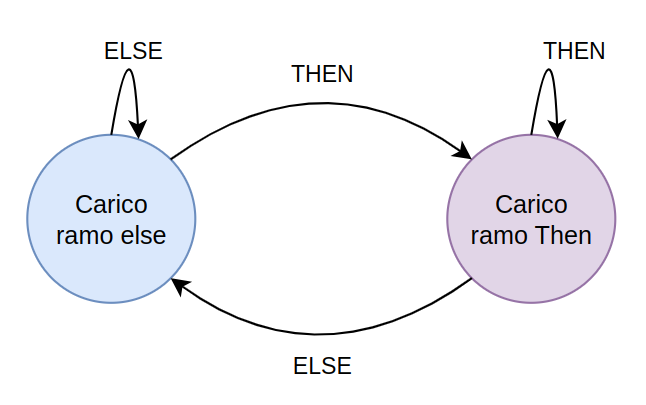
\includegraphics[width=.5\textwidth]{fig/chapter_1/automa-semplice.png}
    \caption{Automa della branch prediction base}\label{img:automa-semplice}
\end{figure}

Questa soluzione non è ottima poichè per quel singolo errore che avviene ad ogni N interazioni la pipeline dovrà assorbire 2 penalties. Per evitare tale condizione, e quindi rendere la persistenza più forte, consideriamo un automa a 4 stati che permette di rendere la condizione di "cambio del branch" più solida, poichè solo in caso di due errori successivi, allora cambio l'indirizzo di salto effettivo. L'automa a cui facciamo riferimento è [\ref{img:automa-complesso}].

\begin{figure}[ht]
    \centering
    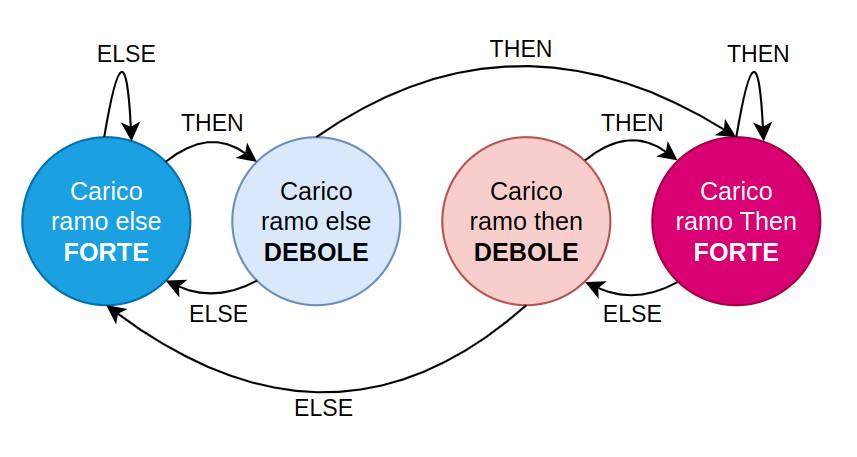
\includegraphics[width=.5\textwidth]{fig/chapter_1/automa-complesso.png}
    \caption{Automa della branch prediction avanzato}\label{img:automa-complesso}
\end{figure}

\noindent Per implementare la predizione a livello hardware, il processore utilizza una \textbf{tabella di predizione} dei salti. Una possibile struttura prevede i campi (Indirizzo dell'istruzione di salto, indirizzo di destinazione, 2 bit per codificare lo stato).

\noindent La tabella viene aggiornata in parallelo durante la fase di Execute (EX), ovvero nel momento in cui il processore verifica se la predizione è corretta. Se c'è stato un errore, si aggiorna lo stato dell'automa (e la corrispondente voce nella tabella). Tale struttura è memorizzata in un apposita area di memoria, detta \textbf{Branch History Table} (BHT).

Con l'introduzione del sistema a pipeline e del meccanismo dell'\textbf{internal forwarding}, che altera la sequenzialità delle istruzioni eseguite dal processore, nasce il problema della \textbf{gestione delle interruzioni}. 
Infatti può capitare che alcune istruzioni siano completate in un ordine diverso da quello in cui sono state avviate. In tal caso è possibile che si generino delle \textit{interruzioni non esatte}, cioè situazioni in cui un' istruzione provoca un' eccezione prima che tutte quelle che la precedono siano completate. Ovviamente, per la corretta gestione delle eccezioni stesse, l'obiettivo che ci si pone è quello di creare un sistema che sia in grado di arrestare opportunamente la pipe in modo da completare le istruzioni che precedono quella che ha generato l'interruzione senza avviare quelle che seguono, così da ottenere un comportamento che rispetti quello descritto dal modello di Von Neumann che viene definito di \textit{gestione precisa} delle interruzioni.
Le \textbf{interruzioni esterne} sono più facili da gestire: infatti la interrupt service routine relativa all'interruzione sopraggiunta verrà inserita nella pipeline come una normale istruzione, dopo che tutte le istruzioni precedenti verranno correttamente terminate, comprese quelle ibernate. 
Più critico è il caso delle \textbf{interruzioni interne}. Infatti questo genere di interruzioni possono essere causate da diverse istruzioni contemporaneamente all'interno della pipe in diversi stages. Non è dunque garantito il comportamento sequenziale di Von Neumann. Un esempio abbastanza lampante di conflitto è il caso in cui nella stessa pipe un'istruzione cerca di effettuare un accesso illegale in memoria (eccezione scatenata nella fase MEM) mentre un'altra istruzione, successiva, tenta una divisione per zero (eccezione scatenata nella fase ID).

\noindent Alcuni processori rinunciano del tutto ad avere interruzioni precise. In questo caso è compito del software assicurare che nella stessa pipeline non ci siano istruzioni le cui possibili eccezioni possano causare questo tipo di conflitto. Considerando il tasso di istruzioni che generano eccezione in un generico codice, questa soluzione può essere più o meno accettabile. Altri processori invece riescono a ricostruire interruzioni precise, utilizzando tecniche di tipo conservativo o ottimistico. 
Nelle tecniche di tipo \textbf{conservativo}, il processore fa procedere nella pipe un'istruzione finché è sicuro che non possa essere fonte di interruzione, e solo a questo punto ne avvia un'altra. Il parallelismo intrinseco della pipe è dunque limitato, a vantaggio della gestione precisa delle eccezioni. 

\noindent Nel caso di tecniche di tipo \textbf{ottimistico}, vengono inserite comunque istruzioni nella pipeline indipendentemente dalla possibilità di generare o meno eccezioni. Se emergono conflitti il sistema deve essere in grado di effettuare un \textit{rollback}, e quindi è necessaria un'immagine dello stato del sistema.  
Il rollback può essere effettuato mediante due tecniche:

\begin{itemize}
    \item \textbf{Check point}: Vengono effettuate periodici snapshot dello stato dei registri del processore, compreso il PC, conservate in una opportuna area di memoria. Nel momento in cui si verifica un'eccezione, vengono ricopiati i valori memorizzati nei registri del processore e si riprende l'esecuzione \textit{sequenziale} del programma, quindi un'istruzione per volta, a partire dall'ultimo valore di PC riportato nello snapshot. Occorre in questo caso scegliere con attenzione la frequenza di cattura dello snapshot. 
    \item \textbf{History Buffer}: Ogni istruzione eseguita viene memorizzata in un'area di memoria insieme ai valori dei propri operandi. Ogni istruzione memorizzata può essere cancelalta dal buffer solo quando tutte quelle che la precedono si sono concluse senza generare interruzione. \uppercase{è} possibile definire in questo modo una sequenza di operazioni UNDO da effettuare nel caso un'istruzione ibernata precedentemente causi un'eccezione. Questa tecnica è anche utile per garantire la gestione precisa delle interruzioni, facendo in modo che un'eccezione non venga gestita se prima non sono terminate correttamente (quindi senza causare eccezioni) le istruzioni ibernate.
\end{itemize}


\section{Problemi nelle architetture superscalari}
\sloppy
Per migliorare le prestazioni di un processore, si può pensare di realizzare un'architettura che presenti più pipe che eseguono diverse istruzioni in parallelo. Questo tipo di architettura viene definito \textbf{superscalare}.
Questa soluzione introduce diverse problematiche.
Una prima problematica riguarda il prelievo delle istruzioni in memoria. Le istruzioni vengono prelevate in maniera sequenziale dalla memoria condivisa, quindi non è possibile che due pipeline inseriscano contemporaneamente in esecuzione due istruzioni diverse. Se le pipeline sono completamente disgiunte, ovvero non condividono alcuna unità funzionale, allora l'unico altro problema è quello relativo alla \textit{branch prediction}. I dispositivi per la predizione del salto devono essere, in questo caso, duplicati. 
Invece se le pipe condividono alcuni stages, la cooperazione e la competizione per le risorse condivise deve essere gestita in maniera più complessa via hardware. 
Quindi non c'è una vera e propria alimentazione in parallelo. Questa condizione di funzionamento, unita alla considerazione che le pipe condividono alcune unità funzionali, ci consente di affermare che il sistema nel suo complesso può essere visto come costituito da una sola pipe con più unità specializzate e con altre che sono in comune.  
Infatti è facile notare che nelle architetture superscalari ciascuna pipe è specializzata 
nell'esecuzione di particolari operazioni.   
Inoltre, per distribuire le istruzioni tra le pipe è possibile pensare di introdurre a monte della fase di EX di ciascuna pipe (dopo le fasi IF e ID) un'unità hardware, detta \textbf{Dispatch}, che analizza più istruzioni per volta e decide quali inserire in quale pipe. Ogni fase di ciascuna pipe, in generale, può essere utilizzata da più pipe per più cicli, quindi risulta particolarmente interessante l'idea di affidare al Dispatch anche il compito di riconoscere le caratteristiche di ciascuna operazione per evitare collisioni tra le pipe.  
Per le sue caratteristiche, la fase di dispatch non può essere realizzata in software, poiché deve essere molto veloce ed efficiente, quindi deve essere necessariamente realizzata in hardware. Strumento fondamentale sia per il compilatore che per il Dispatcher è il \textit{collision vector}, foriero di informazioni utili riguardo la compatibilità temporale di più operazioni che necessitano di condividere la stessa unità funzionale. Per ulteriori dettagli, consultare gli \href{https://github.com/Agda78/APC-appunti}{appunti di APC}.

\chapter{Architetture superscalari dei moderni processori} \label{chap:architetture_superscalari}
\sloppy
Consideriamo una semplice architettura pipeline a cinque stages, costituita da \textit{instruction fetch IF} $\rightarrow$ \textit{instruction decode e operand assemby ID} $\rightarrow$ \textit{Execute EXE} $\rightarrow$ \textit{Memory Load/Store MEM} $\rightarrow$ \textit{Writeback WB}. Ognuno di questi stages logici ha una mappatura diretta con una macchina cambinatoriale dell'architettura del processore.

\begin{info}
Una macchina combinatoriale (o circuito logico combinatorio) è un sistema logico digitale in cui le uscite dipendono esclusivamente dai valori presenti agli ingressi in un dato istante, senza alcuna memoria degli stati precedenti.
\end{info}

\noindent Diverse fasi di diverse istruzioni, come osservato nel capitolo precedente, possono sovrapporsi nel tempo, e il risultato è un incremento del throughput (istruzioni completate/unità di tempo).
\uppercase{è} immediatamente possibile osservare che il tempo di completamento di un'istruzione (in letteratura \textit{latency}) non migliora, anzi al più peggiora, a causa del già discusso overhead introdotto nel controllo della pipeline (Capitolo \ref{chap:richiami_apc}). Il guadagno in termini di throughput idealmente è pari al numero di stadi, ma nella pratica è limitato dall'overhead di pipeline e dagli \textit{hazards}. 

\begin{warn}
Un \textbf{ciclo di clock} è l'unità di tempo fondamentale dettata dal segnale di clock. Tutte le operazioni elementari avvengono in corrispondenza dei fronti di salita del segnale di clock. Un \textbf{ciclo del processore} è il tempo necessario al processore per completare un'operazione base del set di istruzioni. Nelle architetture RISC un ciclo di processore coincide con pochi cicli di clock. Questo tempo viene misurato in \textbf{IPC} (instruction per clock).
\end{warn}

\noindent Quindi in una pipeline il tempo di attraversamento di un'istruzione è leggermente peggiroato principalmente a causa del fatto che la sequenzialità combinatoriale della macchina viene frammentata da registri che hanno bisogno di un tempo di \textit{setup}. Il parametro che ne beneficia è il clock cycle, che rispetto ad una macchina sequenziale, è ridotto a $\frac{1}{N}$ dove N è il numero di fasi in cui viene frammentata la macchina combinatoriale. In realtà il clock non può essere più veloce del più lento stadio combinatoriale, che ne scandisce un limite superiore. La tecnica della pipeline dunque non è facilmente scalabile: I \textit{path} combinatoriali non possono essere arbitrariamente frammentati; inoltre, superata una certa granularità, gli overhead limitano i benefici. \\ \noindent Nel caso reale, nei diversi stages la latenza è variabile. Questo è dovuto al fatto che l'infrastruttura della memoria è complessa e nel caso peggiore potrebbero verificarsi dei \textit{cache miss}, così come il processore potrebbe avere diverse unità funzionali dedicate all'esecuzione, ognuna con la propria latenza (alcune operazioni sono più lunghe e complesse di altre).

\begin{figure}[ht]
    \centering
    \setlength{\fboxrule}{0.5pt} % spessore sottile
    \setlength{\fboxsep}{0pt}    % senza spazio interno
    \fbox{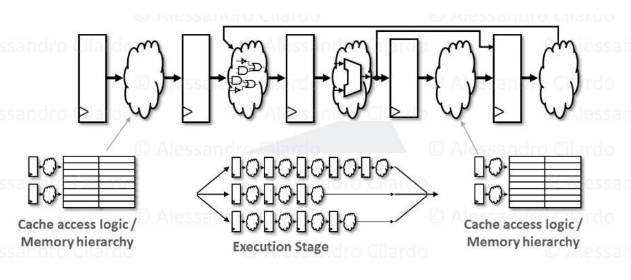
\includegraphics[width=0.6\textwidth]{fig/chapter_2/pipeline_diversity.png}}
\end{figure}

\noindent
Per migliorare l'IPC, si può ricorrere alla moltiplicazione delle istanze di unità funzionali che lavorano in parallelo su più istruzioni. Se l'IPC > 1 si parla di architetture \textbf{superscalari}. \\ \noindent Parlando sempre di pipeline semplice a cinque stadi, possiamo invece agire sull'overhead introdotto dal controllo della pipeline, in particolare risolvere quei conflitti che provocherebbero il blocco (stallo) della pipe. Questo si può fare con l'esecuzione delle istruzioni \textit{out of order}, ovvero con un problema di scheduling vincolato. La pipeline può essere vista nella prospettiva di schedulatore di micro operazioni soggette a vincoli strutturali e dipendenze. I vincoli strutturali sono dettati dell'hardware e scandiscono cosa si può fare in un particolare istante di tempo. I vincoli sulle dipendenze riguardano le relazioni di precedenza tra micro operazioni che devono necessariamente essere soddisfatte nel momento in cui vengono processate dalle unità hardware. 
Rischedulare le micro operazioni può violare i vincoli sulle dipendenze:


\begin{itemize}
    \item \textbf{READ AFTER WRITE (RAW)}: l'operazione di lettura operando di un' istruzione successiva è performata prima dell'operazione di WB sullo stesso registro di un'istruzione precedente;
    \item \textbf{WRITE AFTER WRITE (WAW)}: due istruzioni scrivono lo stesso registro, ma l'ordine di WB è invertito e dunque nel registro si trova un dato vecchio; 
    \item \textbf{WRITE AFTER READ (WAR)}: l'operazione di lettura operando di un'istruzione precedente viene ritardata fino al momento in cui l'operazione di WB di un'istruzione successiva è già avvenuta, distruggendo il contenuto del registro prima che sia letto dall'istruzione precedente.
\end{itemize}



\section{Scheduling statico}
Lo scheduling statico di una pipeline è una tecnica di ottimizzazione usata nei processori con pipelining (soprattutto nelle architetture RISC e VLIW) per ridurre o eliminare i hazard (conflitti di dati, di controllo o strutturali) senza dover ricorrere a meccanismi di risoluzione hardware dinamici. Statico significa che lo scheduling viene fatto dal compilatore, in fase di compilazione, non dal processore a runtime. L'idea è che il compilatore riordini le istruzioni in modo da minimizzare i cicli di stallo (stall) e sfruttare al massimo la pipeline.

\section{Scheduling dinamico}
Con scheduling dinamico intendiamo tecniche hardware che \textit{on the fly}, durante l'esecuzione, cambiano l'ordine di processo di determinate operazioni per risolvere i conflitti ed evitare quando possibile lo stallo della pipeline. I vantaggi di uno scheduling dinamico sono molteplici:

\begin{itemize}
    \item Permette a codice compilato per una determinata architettura di essere efficiente anche su un'architettura diversa, eliminando parzialmente la relazione che sussite tra efficienza e compilazione;
    \item Permette di gestire casi in cui alcune dipendenze non sono note a tempo di compilazione (riferimenti in memoria e salti dipendenti dai dati);
    \item Permette al processore di tollerare dei ritardi non prevedibili a tempo di compilazione (cache miss).
\end{itemize}

Il datapath di una pipeline deve essere gestito da un'opportuna unità di controllo, che risolva potenziali condizioni di \textit{hazard}. Questa unità è responsabile di rilevare il problema e risolverlo bloccando la pipeline a partire da un certo stadio in poi, inserendo delle \textit{bolle}. Per rendere possibile questo controllo è necessario propagare dalla fase ID in poi gli indici deglio operandi, in modo tale che l'unità di controllo possa rilevare possibili conflitti. 

\subsection{Forward paths}
Il vincolo sulla dipendenza RAW riguarda \textit{vere dipendenze}, ovvero dipendenze dettate dal problema produttore-consumatore tra le istruzioni, e sono indipendenti dall'architettura (riguardano in senso logico il flusso di esecuzione del codice). Inserire un path diretto [output ALU $\rightarrow$ registro operandi] permette di rilassare il vincolo di dipendenza e fare in modo che l'unità di controllo possa risolvere il potenziale conflitto.  
In altre parole, si cambia il \textit{grafo delle dipendenze} tra le operazioni.

\begin{figure}[ht]
    \centering
    \setlength{\fboxrule}{0.5pt} % spessore sottile
    \setlength{\fboxsep}{0pt}    % senza spazio interno
    \fbox{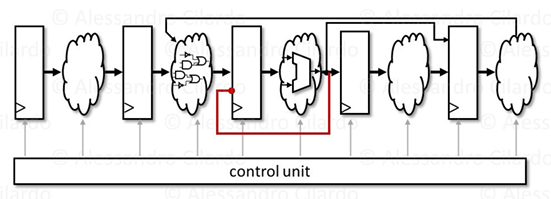
\includegraphics[width=0.6\textwidth]{fig/chapter_2/basic_forwarding.png}}
\end{figure}

\begin{info}
    Grafo delle dipendenze: grafo orientato in cui le istruzioni costituiscono i nodi, gli archi invece rappresentano le dipendenze tra queste.
\end{info}

Il costo di questi benefici è una notevole complicazione dell'hardware. Osserviamo inoltre che lo scheduling dinamico è utlizzabile insieme allo scheduling statico effettuato dal compilatore: una tecnica non prescinde l'altra. \\ \noindent
Osserviamo che in uno schema pipeline a cinque stages di base, dove non contempliamo istruzioni fuori ordine, è verificata sempre la condizione: \textit{una micro-operazione di un'istruzione precedente è sempre eseguita prima della stessa o una successiva micro-operazione di un'istruzione successiva}. In altre parole, se un'istruzione A precede un'istruzione B, l'operazione di \textit{lettura operandi} dell'istruzione A è eseguita prima delle operazioni EX, MEM e WB dell'istruzione B. Di conseguenza, in questo schema semplificato non sono possibili hazards di tipo WAW e WAR. 
Questo è in generale \textbf{falso} per gli approcci basati sul rescheduling delle operazioni. 

\subsection{Esecuzione out-of-order}
Un'unità funzionale, come un moltiplicatore o un divisore, può essere internamente organizzata come una pipeline. In questo modo l'unità può iniziare una nuova operazione ad ogni ciclo, pur impiegando diversi cicli per completare un'operazione. 

\begin{info}
    L'\textbf{initialization interval} (II) è il numero di cicli di clock che devono passare prima di poter avviare una nuova iterazione della pipeline. Questo limite è imposto dall'hardware.
\end{info}

Se l'II dell'unità funzionale serializzata è minore della latenza totale dell'unità, allora più micro-operazioni possono coesistere nella stessa unità funzionale, pur attraversandola sempre in ordine. Se lo stage EXE contiene più di un'unità funzionale specializzata, ognuna con diverse latenze, è necessario introdurre l'esecuzione \textit{out of order}. 
Complicando in questo modo l'hardware, è necessario fare delle considerazioni: differenti unità funzionali possono completare l'esecuzione nello stesso ciclo $\rightarrow$ hazard strutturali sull'insieme dei registri $\rightarrow$ WAW hazard; se l'hardware supporta molteplici operazioni di lettura operandi concorrenti, sono possibili hazards strutturali sullo stage EXE (?); Sono possibili hazard di tipo WAR, e gli hazards ti tipo RAW sono più frequenti. 
Nelle architetture superscalari il processore può emettere ed eseguire più istruzioni nello stesso ciclo di clock. Questo implica che diverse unità funzionali possano aver bisogno, contemporaneamente, di leggere o scrivere registri. Per esempio, due istruzioni aritmetiche emesse nello stesso ciclo possono richiedere entrambe di leggere due operandi e di scrivere un risultato; se il file dei registri fosse accessibile da una sola porta di lettura e scrittura, ci sarebbe un collo di bottiglia che impedirebbe l'esecuzione parallela. Per questo motivo i registri devono essere multiportati, cioè progettati per permettere più accessi simultanei da locazioni diverse, in modo da garantire che le varie istruzioni in issue nello stesso ciclo possano ottenere i loro operandi o aggiornare i risultati senza conflitti. Rendere i registri multiporting è difficile principalmente per ragioni di complessità circuitale e di costo. Ogni porta aggiuntiva di lettura o scrittura richiede linee di accesso dedicate, logica di decodifica separata e soprattutto un incremento del numero di connessioni interne, il che fa crescere in modo quasi quadratico l'area del circuito e la capacità parassita. Questo significa che più porte si aggiungono, più aumenta il consumo energetico e più rallenta il tempo di accesso ai registri.
\\ \noindent Avere a che fare con molteplici scritture implica scegliere una strategia di rilevazione della dipendenza e di risoluzione: se si sceglie di rilevare il conflitto già in fase di ID, il processore deve subito confrontare i registri di destinazione delle istruzioni decodificate con quelli delle istruzioni più vecchie ancora in pipeline. Per non perdere l'informazione man mano che le istruzioni avanzano, si usa una catena di shift registers che traccia la distanza (in termini di stadi di pipeline) fino a quando l'istruzione precedente eseguirà il WB. In questo modo, fin dall'inizio si sa che una certa istruzione dovrà aspettare un certo numero di cicli prima di poter scrivere in sicurezza. Il vantaggio è che i conflitti sono gestiti in anticipo, evitando bolle tardive. Lo svantaggio è che servono comparatori e logica aggiuntiva in ID, e gli shift register complicano l'hardware.
L'alternativa è rilevare il conflitto il più tardi possibile, cioè attendere che le istruzioni arrivino in prossimità della fase di write-back e solo lì controllare se due istruzioni stanno tentando di scrivere lo stesso registro nello stesso ciclo. Questo riduce la complessità logica in ID e alleggerisce la pipeline nei primi stadi, ma aumenta la probabilità di dover bloccare o annullare (stall o flush) istruzioni già avanzate nella pipeline. In altre parole: hardware più semplice, ma più penalità in caso di conflitti.
In generale conviene rilevare i conflitti presto (in ID con shift register) quando si ha un'architettura aggressivamente superscalare o molto profonda, dove i conflitti diventano frequenti e lo stall tardivo sarebbe molto costoso.
Gli hazard possono essere significativamente ridotti introducendo \textbf{isolated type registers}. Ciò significa che, invece di avere un unico file di registri condiviso da tutte le unità funzionali, il processore suddivide i registri in più gruppi separati, ciascuno dedicato a un certo “tipo” di istruzione o unità. Per esempio, ci possono essere registri isolati per le operazioni intere, altri per le operazioni in virgola mobile etc. La separazione riduce drasticamente le probabilità di conflitto, perché istruzioni appartenenti a domini funzionali diversi non competono per lo stesso insieme di registri. Inoltre, avere registri specializzati permette anche di ridurre la complessità del multiporting, dato che ogni file di registri isolato può essere più piccolo e più facile da gestire in parallelo.
\\
L'idea chiave è separare la fase ID in due fasi indipendenti, \textbf{instruction issue} e \textbf{operand read}. L'instrucion issue consiste nell'\textit{accettare} l'istruzione, riservando risorse per tracciarla in stages successivi, e ciò viene di solito performato \textit{in ordine}; l'operand read invece aspetta che gli operando siano pronti, ed è tipicamente performate \textit{out of order}.

\begin{figure}[ht]
    \centering
    \setlength{\fboxrule}{0.5pt} % spessore sottile
    \setlength{\fboxsep}{0pt}    % senza spazio interno
    \fbox{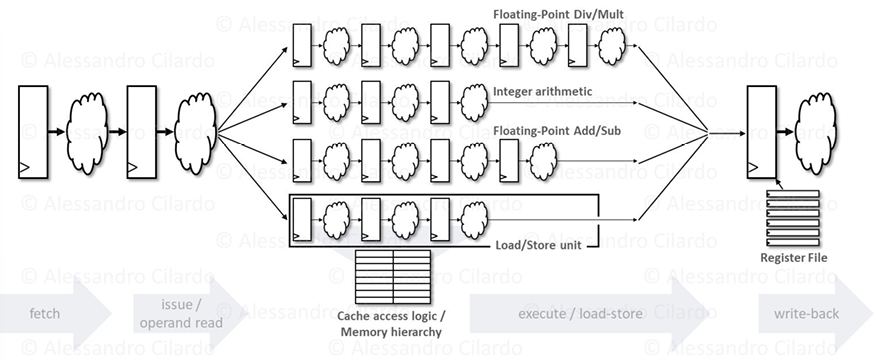
\includegraphics[width=0.6\textwidth]{fig/chapter_2/out_of_order.png}}
\end{figure}

Nella trattazione teorica qui presentata conviene trattare l'unità di load/store (MEM) come un'unità funzionale al pari delle unità funzionali dedite alle operazioni aritmetico-logiche. 

\subsection{Scoreboard}
In questa tecnica di implementazione dell'unità di controllo facciamo delle assunzioni: 
\begin{itemize}
    \item L'issue di un'istruzione ovviene in ordine, e in questa fase vengono rilevati hazards strutturali e WAW;
    \item L'operand read avviene, così come la fase EX e la fase di completamento, out-of-order. Inoltre le dipendenze sui dati sono risolte dinamicamente;
    \item Non vi sono espliciti forwarding paths;
    \item Per ora ci disinteressiamo del modello delle eccezioni/interruzioni.
\end{itemize}

La logica per le fasi issue e operand read sono gestite attraverso due tabelle (\textbf{unit status table} e \textbf{register status table}) dall'unità di controllo.

\begin{figure}[ht]
    \centering
    \setlength{\fboxrule}{0.5pt} % spessore sottile
    \setlength{\fboxsep}{0pt}    % senza spazio interno
    \fbox{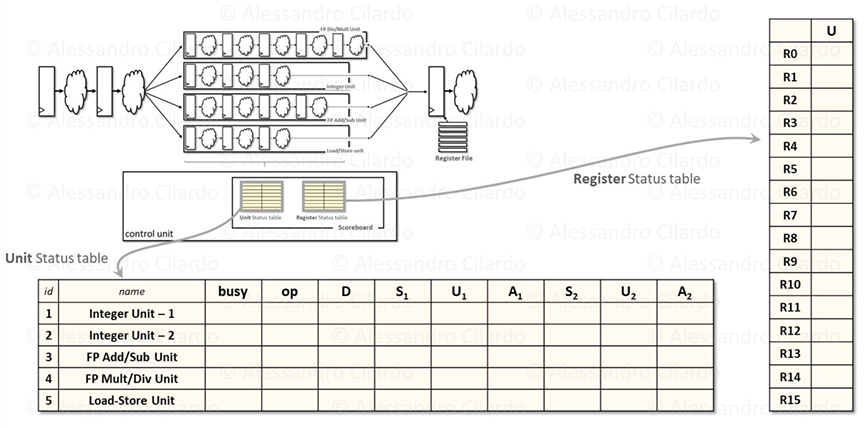
\includegraphics[width=0.6\textwidth]{fig/chapter_2/scoreboard.png}}
\end{figure}

\noindent La unit table ha tante righe quante le unità funzionali e i seguenti campi:

\begin{description}[style=nextline,leftmargin=3.45cm,labelwidth=2.8cm,labelsep=0.4cm,font=\ttfamily\bfseries, itemsep=0.01em]
\item[id] Intero che identifica l'unità funzionale
\item[name] Nome dell'unità funzionale
\item[busy] Flag che indica se l'unità è occupata
\item[op] Specifica operazione righiesta all'unità funzionale 
\item[D] Indice del registro destinazione 
\item[$S_i$] Indice dell'i-esimo registro sorgente    
\item[$U_i$] Id dell'unità che eventualmente sta processando il valore che sarà scritto in $S_i$ (=0 se è già disponibile)
\item[$A_i$] Flag che verifica se il valore nel registro è già disponibile per la lettura  
\end{description}

\noindent Per quanto riguarda la Register Status Table, questa ha tante riche quanti sono i registri e l'unico campo U $\rightarrow$, che contiene l'id dell'unità che evnentualmente sta processando il valore che verrà scritto nel registro (=0 se già disponibile).
\\ \noindent Le istruzioni sono recuperate dalla pipeline in ordine e poi possono trovarsi in una delle seguenti fasi: Issue, Operand Read, Execute o Write Back. 
Le regole per aggiornare le tabelle sono queste:

\begin{itemize}
    \item Un'istruzione viene \textit{accettata} (issued) solo se:
    \item \begin{itemize}
        \item L'unità funzionale richiesta è libera (free = 0);
        \item Il 
    \end{itemize}
\end{itemize}


\section{Dipendenze di controllo}
Per massimizzare l'efficienza di un processore devono verificarsi meno \textit{pipe flush} possibili e ridurre al minimo l'inserimento di bolle. Le dipendenze di controllo si riferiscono a situazioni in cui nel codice è presente un salto. Ciò accade molto frequentemente, infatti circa una ogni quattro istruzioni prevede un salto. Questo è problematico perche idealmente il grafo di esecuzione si sdoppia, ed è praticamente impossibile sfruttare il parallelismo intrinseco delle istruzioni non conoscendo a priori quali istruzioni caricare. In sintesi, i salti rendono il flusso dati \textit{dinamico}: le assegnazioni sono condizionali. Idealmente, le dipendenze di controllo possono essere eliminate linearizzando il flusso di esecuzione del codice. Questo si può fare solo sotto l'ipotesi di predizione del salto perfetta e sotto l'ipotesi che tra un branch e l'altro ci siano sufficienti istruzioni. 

\begin{figure}[ht]
    \centering
    \setlength{\fboxrule}{0.5pt} % spessore sottile
    \setlength{\fboxsep}{0pt}    % senza spazio interno
    \fbox{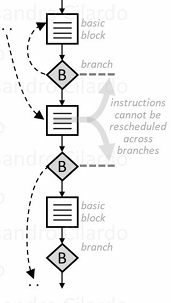
\includegraphics[width=0.28\textwidth]{fig/chapter_2/control_dependencies.png}}
\end{figure}


\noindent La predizione del branch a cui saltare però nella pratica non è mai perfetta, e avviene tramite meccanismi hardware (quelli di base sono descritti nel paragrafo [\ref{subsec:control_hazards}]) e software, come l'inserimento di un bit di indizio staticamente inserito nell'istruzione. Osserviamo che poichè il branch predictor \textit{scommette} sulla prossima istruzione da caricare, non fermando mai la pipeline, sono necessari meccanismi di \textbf{commit} o \textbf{rollback} per non comporomettere in maniera irreversibile lo stato del processore o peggio ancora della memoria. 

\subsection{Generalizzazione predittore a 2 bit}
Un predittore dinamico (hardware) a due bit è posizione a monte della fase issue. Il suo scopo è associare ad ogni istruzione di salto una predizione, ovvero un indirizzo target. Questo avviene consultando una memoria associativa, la cui chiave è un sottoinsieme dei bit dell'istruzione di salto. 

\begin{warn}
    di solito per indicizzare la branch history table si usano i bit meno significativi dell'istruzione di salto. Questo perchè si vuole mantenere contenuta la dimensione spaziale della tabella senza implementare meccanismi di decodifica o di hashing. Ciò significa eventualmente accettare collisioni, ma questo è un problema solo di performance, risolvibile e tollerabile se sufficientemente raro. Infatti i cambiamenti allo stato della memoria e del processore diventano effettivi solo quando la condizione del salto viene calcolata in fasi più avanzate della pipeline.
\end{warn}

I predittori a due livelli introducono un inerzia nel cambio di decisione per massimizzare l'efficienza nel caso di due loop innestati. Questa tecnica può essere generalizzata. Infatti è possibile costruire predittori a n bit, rendendo disponibili $2^n$ stati per la decisione e potendo arbitrariamente scegliere una tra le transizioni di stato che generano il cambio di decisione.  

\begin{figure}[ht]
    \centering
    \setlength{\fboxrule}{0.5pt} % spessore sottile
    \setlength{\fboxsep}{0pt}    % senza spazio interno
    \fbox{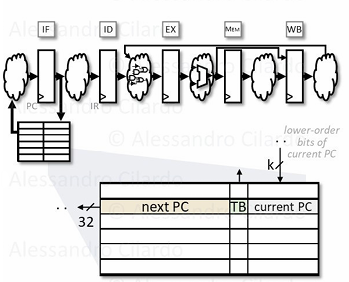
\includegraphics[width=0.45\textwidth]{fig/chapter_2/n_bit_predictor.png}}
\end{figure}


\noindent Succede spesso che l comportamento di un branch sia correlato a quello di diversi altri branch presenti nel codice. L'informazione sull'esito dei branch correlati può essere utile nel determinare la predizione. Si può pensare quindi di rendere la predizione locale dipendente dalla storia \textit{globale} dei salti, ovvero dal comportamento degli ultimi m salti, indipendentemente da dove si trovavano nel codice (per questo globale). \uppercase{è} naturale quindi implementare questa \textit{storia} come uno shift register a m bit.  
Così si costruiscono meccanismi hardware, denominati (m,n)-predittori, che in base al comportamento globale scelgono una delle $2^m$ branch history tables da consultare. Questo meccanismo è veloce ed efficace, ma richiede diverse iterazioni per andare a regime. Quindi è ragionevole usarlo in caso di molte iterazioni che coinvolgono diversi salti. Osserviamo che questo meccanismo approssima una tecnica di machine learning di \textit{addestramento} per una predizione. 

\begin{warn}
    Il numero di branch history tables da consultare cresce esponenzialmente con m, quindi bisogna cercare un trade off tra efficienza e consumo di risorse.  
\end{warn}

\begin{figure}[ht]
    \centering
    \setlength{\fboxrule}{0.5pt} % spessore sottile
    \setlength{\fboxsep}{0pt}    % senza spazio interno
    \fbox{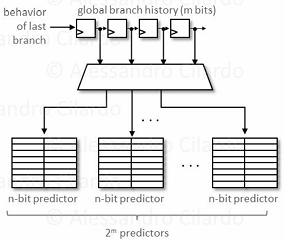
\includegraphics[width=0.45\textwidth]{fig/chapter_2/predittore_m_n.png}}
\end{figure}

\noindent Alcune tecnologie mirano all'implementazione di un predittore di indirizzo, oltre che ad un predittore di esito del salto. Questo è utile in casi come istruzioni di ritorno da subroutine, in cui il campo \textit{next PC} non è noto staticamente, ma deve essere recuperato nello stack. In alcuni processori moderni viene contemplata l'esistenza di una stack utilizzata soltanto per contenere indirizzi di ritorno, in modo da semplificare e velocizzare il recupero (questa memoria è alla base di molti attacchi di tipo \textit{code injection}). 

\begin{info}
    i problemi di indirizzo determinato dinamicamente possono essere risolti staticamente da software, attraverso le espansioni \textit{inline} delle funzioni, in modo da determinare a tempo di compilazione (sfruttando meccanismi di memoria virtuale) l'indirizzo a cui saltare.  
\end{info}

\subsection{Gestione delle eccezioni}
Nel modello di esecuzione out of order, le eccezioni possono occorrere in uno stage qualsiasi della pipeline. Per un richiamo su come vengono gestite le eccezioni in una pipeline semplice a cinque stadi, consultare il paragrafo [\ref{subsec:control_hazards}].

\noindent Per quanto riguarda l'approccio speculativo, è possibile permettere alle istruzioni di procedere fino alla fase di WB, anche quando non è sicuro che debbano essere eseguite. Chiaramente serve un meccanismo di ripristino qualora la speculazione fosse sbagliata. La speculazione hardware ha quindi bisogno di una fase \textit{commit} aggiuntiva. 
Il workflow diventa \textbf{issue} (in order) $\rightarrow$ \textbf{OpRead, EXE, WB} (out of order) $\rightarrow$ \textbf{commit} (in order).
Le istruzioni possono leggere risultati ancora non commitati da istruzioni precedenti, attraverso un buffer temporaneo, non direttamente dai registri. 

\noindent Una particolare tecnica utilizzata per la speculazione hardware è il \textbf{Re-Order Buffer} (ROB). Questo buffer traccia le istruzioni complete ma non committate e mantiene gli operandi di queste istruzioni tra il completamento e il commit. Usato in combinazione con lo schema di Tomasulo, i dati sono bufferizzati anche all'interno delle Reservation stations tra la fase di issue ed execute. 

\begin{figure}[ht]
    \centering
    \setlength{\fboxrule}{0.5pt} % spessore sottile
    \setlength{\fboxsep}{0pt}    % senza spazio interno
    \fbox{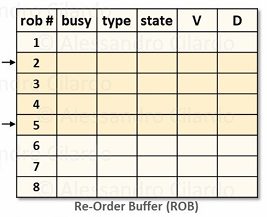
\includegraphics[width=0.5\textwidth]{fig/chapter_2/ROB.png}}
\end{figure}

\noindent I campi del ROB hanno il seguente significato:

\begin{description}[style=nextline,leftmargin=3.45cm,labelwidth=2.8cm,labelsep=0.4cm,font=\ttfamily\bfseries, itemsep=0.01em]
\item[rob \#] Identifica le operazioni 
\item[type] usato per distinguere le operazioni di store e tracciare i salti 
\item[state] Flag che indica se il campo V è valido 
\item[D] Registro target in scrittura 
\item[V] Valore da scrivere nel registro   
\end{description}

\noindent Le Reservation Station subiscono delle modifiche, in particolare i campi $S_i$ vengono sostituiti dalle entry $rob_i$, mentre il campo D viene sostituito da $D_rob$. Analogamente la status register table conterrà due campi per ogni registro (busy, rob) in cui viene indicato se una particolare operazione aspetta di effettuare il commit di una scrittura su quel particolare registro.  
\section{Multiple issue}
Il Multiple Issue è la capacità fondamentale delle moderne CPU superscalari di prelevare, decodificare ed accettare più istruzioni contemporaneamente nello stesso ciclo di clock. Per sostenere questo parallelismo, l'architettura interna necessita di un potenziamento significativo: bisogna allargare il bus degli operandi per gestire il trasferimento simultaneo di dati e potenziare la logica di emissione e scheduling delle istruzioni. Il processo è estremamente rapido e prevede l'assegnazione preventiva delle risorse necessarie e una meticolosa analisi delle dipendenze tra tutte le istruzioni candidate all'emissione, al fine di evitare conflitti di dati (RAW, WAW, WAR). L'implementazione hardware è complessa perché le tabelle di stato interne che tracciano l'uso delle risorse (come i registri e le unità funzionali) devono essere aggiornate in parallelo per l'intero bundle di istruzioni e completare il tutto in un solo ciclo di clock. Inoltre, il controllo delle dipendenze tra più istruzioni richiede un numero massivo di operazioni di confronto eseguite in parallelo, generando un notevole overhead logico. È difficile superare le quattro istruzioni emesse per ciclo perché l'aumento della complessità logica e il conseguente ritardo sul clock spesso superano i guadagni di prestazione. Questa soglia è critica anche perché la speculazione (l'esecuzione predittiva) deve continuare a funzionare in modo efficiente; gestire troppe istruzioni speculative in contemporanea aumenta drasticamente il costo di un errore di predizione. Per migliorare l'efficienza, una strategia comune è separare le istruzioni intere da quelle in virgola mobile, permettendo un scheduling più flessibile e l'uso di unità funzionali dedicate. Altre unità di supporto giocano un ruolo cruciale: un'unità di prelievo (fetch) efficiente con un'unità branch integrata per la predizione dei salti e la disponibilità di più linee di cache L1 aiutano a mantenere il flusso di dati e istruzioni. Le sfide aggiuntive includono l'elevato consumo energetico derivante dall'attivazione parallela di molteplici componenti, la penalizzazione causata dai mancati accessi alla cache che possono bloccare interi bundle di istruzioni, e la complessità di gestire più istruzioni di salto speculative nello stesso ciclo di emissione.

\begin{figure}[ht]
    \centering
    \setlength{\fboxrule}{0.5pt} % spessore sottile
    \setlength{\fboxsep}{0pt}    % senza spazio interno
    \fbox{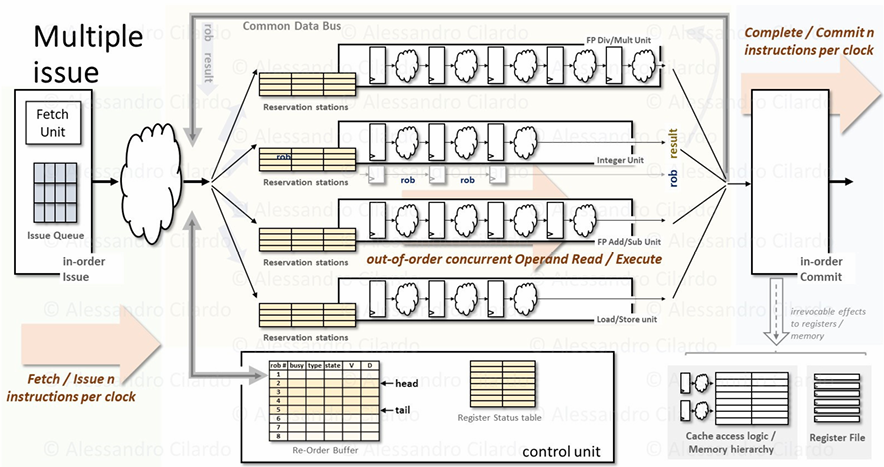
\includegraphics[width=0.75\textwidth]{fig/chapter_2/multiple_issue.png}}
\end{figure}

\noindent Il parallelismo interno è possibile grazie alle tecniche hardware e software fin qui presentate; viene demandata al programmatore, tramite il supporto hardware, l'espressione di ulteriore parallelismo.

\end{document}